\chapter{کارهای پیشین}

\section{الگوریتم‌های کلاسیک تولید موسیقی}

از همان ابتدای پیدایش کامپیوترهای امروزی، موسیقی‌دان‌ها در تلاش برای تولید ملودی‌های جدید به وسیله‌ی کامپیوترها بوده‌اند.
مثال‌هایی از تلاش‌ها برای تولید موسیقی به وسیله‌ی محاسبات کلاسیک در زیر آمده‌اند:

\begin{itemize}
    \item 
    در دهه‌ی ۴۰ میلادی، پژوهشگران مجمع علمی-صنعتی استرالیا
\fnote{Australian council for scientific and industrial research (CSIR)}
بلندگویی را به یک کامپیوتر ام‌کا۱
\fnote{MK1}
متصل کردند تا صدایی که کامپیوتر در حین اجرای برنامه‌ها تولید می‌کرد را بشنوند. در همین راستا و در سال ۱۹۵۱، جف هیل
\fnote{Geoff Hill}
که ریاضی‌دانی با پیش‌زمینه‌ای در موسیقی بود، برنامه‌ای بر روی این کامپیوتر اجرا کرد تا صدای تولید شده تا حد بسیار خوبی شبیه ملودی‌های موسیقی شود.
\cite{CSIR_music}

\item
مدل‌های ترجمه‌ای
\fnote{Translational models}
سعی می‌کنند تا داده‌های غیرصوتی را به صوت تبدیل کنند؛ به عنوان مثال اگر مدلی ساخته شود که سعی کند عکس‌های با فرمت 
\lr{jpg}
را به فایل‌هایی با فرمت
\lr{mp3}
تبدیل کند (چرا که هر دوی این فرمت‌ها برای ذخیره‌سازی، از تبدیل فوریه استفاده می‌کنند)؛ ممکن است عکس یک خط صاف را به عنوان یک موسیقی با یک نت ثابت تعبیر کند

\item
مدل‌های گرامری
\fnote{Grammatical models}
سعی می‌کنند با پردازش کردن داده‌های موسیقیایی به عنوان جملات زبانی که همانند زبان طبیعی، از قواعد گرامری خاصی تبعیت می‌کند؛ الگوریتم‌های پردازش زبان طبیعی
\fnote{Natural Language Processing (NLP)}
را بر روی داده‌های موسیقیایی اعمال کنند.

\item
متدهای تکاملی، با استفاده از چهارچوب الگوریتم‌های ژنتیک
\fnote{Genetic algorithms}
؛ با یک سری از نت‌های موسیقی به عنوان ژن افراد یک جمعیت برخورد می‌کنند و بعد از ترکیب کردن ژن‌های این افراد و ایجاد جهش‌های تصادفی در این ژن‌ها، موسیقی‌های جدیدی تولید کنند.
به عنوان مثال، یک الگوریتم ژنتیک ممکن است دو گام زیر را به این صورت ترکیب کند:
\begin{equation}
\begin{gathered}
    C_{major} = [C, D, E, F, G, A, B, C]\\[3pt]
    A_{major} = [A, B, C\sharp, D, E, F\sharp, G\sharp, A] \\
    Genetic(A_{major}, C_{major}) = [C, D, E, F, E, F\sharp, G\sharp, C] 
\end{gathered}
\end{equation}
\myequations{خروجی الگوریتم ژنتیک بر روی دو گام موسیقی}
که نیمه‌ی اول گام 
$C_{major}$
با نیمه‌ی دوم گام
$A_{major}$
ترکیب شده‌است و نت آخر از 
$A$
به
$C$
جهش یافته‌است.

\item 
با پیدایش و همه‌گیر شدن حوزه‌های هوش مصنوعی و یادگیری ماشین، مدل‌های یادگیری ماشین زیادی برای تولید موسیقی پیشنهاد شده است.
کتاب‌خانه‌ی 
\lr{Magenta}
که توسط بخشی از تیم کتاب‌خانه‌ی یادگیری ماشین
\lr{TensorFlow}
توسعه یافته‌است، شامل پیاده‌سازی انواع مختلفی از این مدل‌ها، از جمله
\lr{Melody RNN}
\cite{magenta_melodyrnn}
و
\lr{GANSynth}
\cite{magenta_gansynth}
است. مدل اول با استفاده از نوع خاصی از حافظه‌های طولانی کوتاه-مدت
و نوع دوم با استفاده از نوع خاصی از شبکه‌های زایای دشمن‌گونه اقدام به تولید موسیقی‌های بدیع می‌کند.
\end{itemize}

\section{الگوریتم‌های کوانتومی تولید موسیقی}

در سال‌های اخیر و با همه‌گیر تر شدن حوزه‌های کوانتومی، چندین پیشنهاد برای بررسی ارتباط بین این حوزه و موسیقی پیشنهاد شده‌است. منبع
\cite{Putz_quantum_music}
برای اولین بار، بررسی تولید موسیقی کوانتومی
\fnote{Quantum music}
و به‌طور کلی‌تر، هنرهای کوانتومی
\fnote{Quantum arts}
را مطرح کرد؛ ایده‌ی اصلی این مقاله این است که در صورتی که بتوان در دنیای روزمره، موج‌های کوانتومی‌ای تولید کرد که بتوانند از نویزهای محیط در امان بمانند؛ می‌توان موج کوانتومی‌ای تولید کرد که در وضعیت برهم‌نهی از دو موسیقی متفاوت باشد. در صورت تحقق این امر، در هنگام شنیده‌شدن این موج توسط گوش انسان، عمل اندازه‌گیری انجام می‌گیرد و به همین خاطر، هر شنونده موسیقی متفاوتی می‌شنود.
این مقاله، منجر به پروژه‌ی
\lr{Quantum Music}
\cite{quantum_music_event}
شد که مقالات منتشر شده در راستای این پروژه، ایده‌های الهام گرفتن از معادلات موج کوانتومی برای تولید موسیقی
\cite{Helweg_QInspired_Music}
و استفاده از تصادفی‌بودن نتایج اندازه‌گیری در محاسبات کوانتومی و بازپخت کوانتومی
\fnote{Quantum annealing}
برای تولید موسیقی
\cite{Kirke_QC_Music}
را به صورت ابتدایی بررسی می‌کنند.

در نهایت، منبع
\cite{miranda}
روش استفاده گشت گراف کوانتومی
\fnote{Quantum Walk}
برای تولید موسیقی را پیشنهاد می‌کند.

مساله‌ی گشت گراف کوانتومی، معادل کوانتومی مساله‌ی گشت گراف کلاسیک است؛ به این معنا که یک موجود ریاضیاتی به نام گردش‌گر
\fnote{Walker}
در یکی از ندهای یک گراف قرار می‌گیرد، به صورتی که حرکت این موجود در گراف، تابع قوانین خاصی است. هدف این گونه مسائل، آنالیز مسیرهای طی شده توسط این موجود و توزیع احتمالاتی
\fnote{Probability distribution}
مکان نهایی آن در گراف بعد از گذشت زمان مشخصی است.
اما به خاطر تفاوت‌های موجود بین این دو حوزه، نتایج آن‌ها نیز متفاوت است.
\cite{Kempe_qwalk}
به عنوان مثال، رابطه‌ی انحراف معیار
\fnote{Standard deviation}
($\sigma$)
توزیع احتمالاتی گشت با تعداد گام‌های طی‌شده
($T$)
در حالات کلاسیک و کوانتوم به شکل زیر متفاوت است:
\begin{equation}
\begin{gathered}
    \sigma^2_{Classical} \sim T \\[3pt]
    \sigma^2_{Quantum} \sim T^2
\end{gathered}
\end{equation}

\begin{figure}
	\centering
	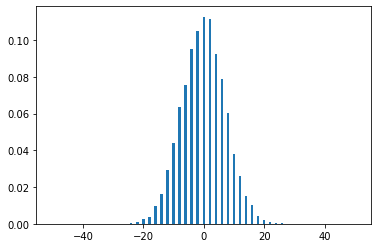
\includegraphics[scale=0.5]{figures/classical_distribution.png}
	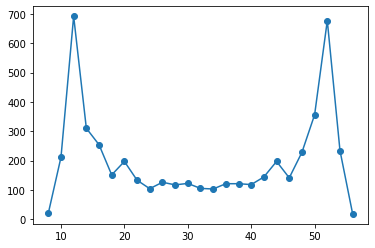
\includegraphics[scale=0.5]{figures/quantum_distribution.png}
	% To make sure citation doesn't appear in list of figures
	\caption [
	مقایسه‌ی توزیع احتمالی گشت گرافی کلاسیک و کوانتوم
	]{
	مقایسه‌ی توزیع احتمالی گشت گرافی کلاسیک (راست) و کوانتومی (چپ)
	\cite{cirq_qwalk}
	}
	\label{fig:walk_distr}
\end{figure}

\myequations{انحراف معیار گشت‌های کوانتوم و کلاسیک}
به طور خلاصه، الگوریتم گشت گراف کوانتومی، وضعیت گردش‌گر را در چند کیوبیت کدگذاری می‌کند و با فرض شروع مسیر گردش‌گر از یک ند خاص در گراف؛ در هر مرحله، با استفاده از یک کیوبیت سکه
\fnote{Coin qubit}
که در هر مرحله تحت تاثیر یک گیت هادامارد قرار می‌گیرد، وضعیت کیوبیت‌ها را به برهم‌نهی‌ای از وضعیت ندهای مجاور آن گراف می‌برد. نکته‌ای که باعث تفاوت حرکات گردش‌گر کلاسیک و کوانتومی می‌شود، اثر تداخل کوانتومی
\fnote{Quantum interference}
است که احتمالات حضور گردش‌گر در برخی نت‌ها را تقویت و در برخی دیگر، تضعیف می‌کند.
مقایسه‌ی توزیع احتمال مکان نهایی گردش‌گر در اجرای الگوریتم گشت بر روی گراف حلقوی‌ای با ۶ ند در حالت کلاسیک و در حالت کوانتومی‌ای که کیوبیت سکه‌ی آن در زمان
$t=0$
از وضعیت اولیه‌ی زیر شروع شده:
\begin{equation}
    |i\rangle = \frac{|0\rangle + i|1\rangle}{\sqrt{2}}
\end{equation}
\myequations{وضعیت اولیه‌ی کیوبیت‌ها در یک گشت کوانتومی}
در شکل
\ref{fig:walk_distr}
آمده است.
بیان ریاضی عمل‌گرهای الگوریتم گشت کوانتومی به صورت زیر است:
\begin{equation}
\begin{gathered}
    |q_t\rangle = |state_t\rangle \otimes |coin_t\rangle \\[3pt]
    U = |0\rangle \langle 0| \otimes \sum_j |j + 1\rangle \langle j| + |1\rangle \langle 1| \otimes \sum_j |j - 1\rangle
    \langle j| \\[3pt]
    S = U(H \otimes \mathbb{I}) \\[3pt]
    |q_{t+1}\rangle = S|q_t \rangle
\end{gathered}
\end{equation}
\myequations{بیان ریاضی عمل‌گرهای الگوریتم گشت کوانتومی}

که منظور از بردارهایی به شکل
$|j\rangle$
و 
$|j+1\rangle$
نمایش وضعیت کیوبیت‌های بردارهای وضعیت به شکل عدد طبیعی است که عمل‌گرهای جمع و تفریق حلقوی به آن‌ها اعمال می‌شود؛ به عنوان مثال:
\begin{equation}
    \begin{gathered}
        |7\rangle = |111\rangle \\[3pt]
        |7 + 1\rangle = |8 \hso mod \hso 8\rangle = |0\rangle = |000\rangle \\[3pt]
        |0 - 1\rangle = |-1 \hso mod \hso 8\rangle = |7\rangle = |111\rangle
    \end{gathered}
\end{equation}
\myequations{مثال عمل‌گرهای جمع و تفریق حلقوی در الگوریتم گشت کوانتومی}

الگوریتم پیشنهاد شده در 
\cite{miranda}
نمونه‌گیری از یک الگوریتم گشت کوانتومی روی یک گراف با ۸ ند است که تنها به ۳ کیوبیت نیاز دارد. این الگوریتم پس از اندازه‌گیری وضعیت گردش‌گر گراف در انتهای چند مرحله گشت، وضعیت
$|000\rangle$
را به عنوان سکوت، و ۷ وضعیت پایه‌ی دیگر را به عنوان ۷ نت ماژور (معادل کلیدهای سفید پیانو) در نظر می‌گیرد و بر اساس چندین بار اجرای این الگوریتم، قطعه‌ای در یک کلید ماژور تولید می‌کند.